\documentclass[hidelinks, 12pt, oneside]{article}
\usepackage{graphicx}
\usepackage{bookmark}
\usepackage{hyperref}
\usepackage{epsfig}
\usepackage{epstopdf}
\usepackage{caption}
\usepackage{listings}
\usepackage{float}


%\graphicspath{{}}
\begin{document}
 
%titlepage
\thispagestyle{empty}
\begin{center}
\begin{minipage}{0.75\linewidth}
    \centering
%University logo
    
\includegraphics[width=13cm]{./graphics/universityLogo.jpg}
    \rule{0\linewidth}{0.15\linewidth}\par

%Thesis title
    {\uppercase{\Large Project Storm \par}}
    {\uppercase{\Large Functional Requirements Specification \par}}
   	{\uppercase{\Large Team NAME \par}}
    \vspace{1cm}
%Author's name
    {\normalsize Renaldo van Dyk 12204359\par}
    {\normalsize Sean Hill 12221458\par}
    {\normalsize Shaun Meintjes 133310896\par}
    {\normalsize Johann Dian Marx 12105202\par}

    \vspace{0.7cm}
	{\Large Client: \par}
	{\normalsize Linda Marshall \& Vreda Pieterse \par}
	{\normalsize  lmarshall@cs.up.ac.za,vpieterse@cs.up.ac.za\par}
	\vspace{0.7cm}
    \vspace{1cm}
    
    \href{https://github.com/DianMarx/STORM}{GitHub link}
    \vspace{1cm}
	
\end{minipage}
\end{center}
\clearpage

\tableofcontents
\newpage
\section{Vision and Scope}
\subsection{History and Background}
\subsubsection{A Brief History of Project STORM}
In 2013 lecturers of the department of Computer Science, which resides at the University of Pretoria,
approached honors students of the module ``Educational Software Development'' to develop a team
shuffling system. 
The system was going to be used by the lecturers of the module ``Software Engineerin'' to
determine teams for the ``Rocking the boat'' exercise of the ``Software Engineering'' module using a
set of lecturer defined criteria to select the teams with. An incomplete requirements specification document
was designed and the project was brought to an end. 

\subsubsection{Project Background}
The lecturers of the ``Software Engineering'' module sought the need for such a shuffling tool, this
time approaching students of the ``Software Development'' module. The requirements specification previously 
developed will be used as a starting point. This document will be stripped down to a ``basic system'' requirements
specification, not completely discarding functionality specified in the previous documentation but adding relevant functionality
as the development life-cycle persists.

\subsection{Project Scope}
The complete system should enable users to build teams, from a list of students, by selecting a
set of criteria. This will aid the users in such a way that the users do not have to build the teams
manually, which may require a lot of time. The users can spend their time rather on analyzing
the results of each ``Rocking the Boat'' round to change the criteria for the next round more
effectively.


\section{Application requirements and design}
\subsection{Modular Design}


\begin{flushleft}
The system is to be a modular system which allows for:
\end{flushleft}

\begin{itemize} 
\item[$\bullet$] Only a subset of modules to be deployed. Minimally the system will require the core modules to be deployed.
\item[$\bullet$] Further modules to be added at a later stage.
\end{itemize}

\begin{flushleft}
To this end there should be:
\end{flushleft}

\begin{itemize} 
\item[$\bullet$] Minimal dependencies between modules, and
\item[$\bullet$] No dependencies of core modules on any add-on modules.
\end{itemize}

\begin{flushleft}
Modular design allows that each module encapsulates information that is not available to the rest of the program. This information hiding reduces the cost of subsequent design changes when future functionality is added to STORM. For example, if at a later stage functionality is added to allow for personality tests to be completed within STORM and results are automatically pulled in, a new module can be added without affecting other modules.
\end{flushleft}

\begin{figure}[h]
\centering
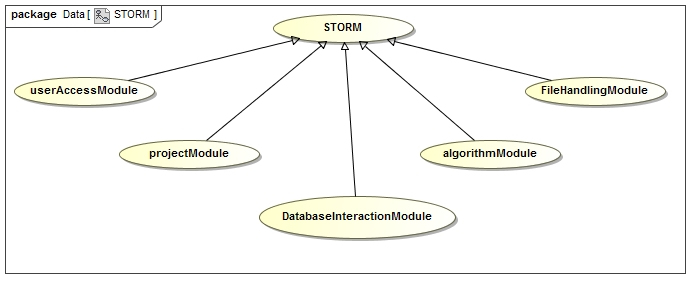
\includegraphics[width=15cm]{./graphics/stormOverview.jpg}
\caption{High level overview of STORM}
\end{figure}
\subsection{User Access Module}
This module deals with the STORM user access, specifically signing up, logging in, logging out and user authentication.

\subsubsection{Use-cases}
\begin{figure}[H]
    \centering
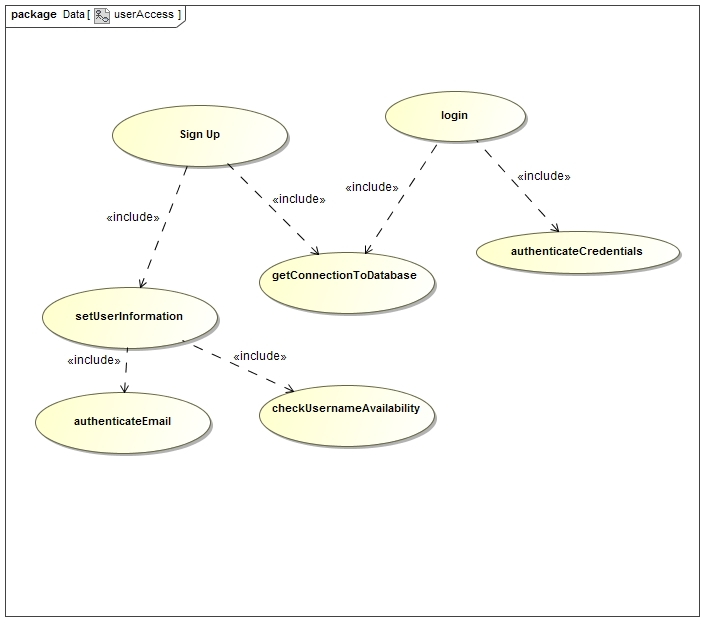
\includegraphics[width=15cm]{./graphics/userAccessUseCase.jpg}
    \caption{ User access module use case}
\end{figure}

    \rule{0\linewidth}{0.15\linewidth}\par
\begin{enumerate}
\item Sign Up\par
Priority: Critical.\par
Pre-condition: Client must have a valid e-mail address.\par
Post-condition: Client has a STORM profile.\par
\begin{figure}[H]
    \centering
    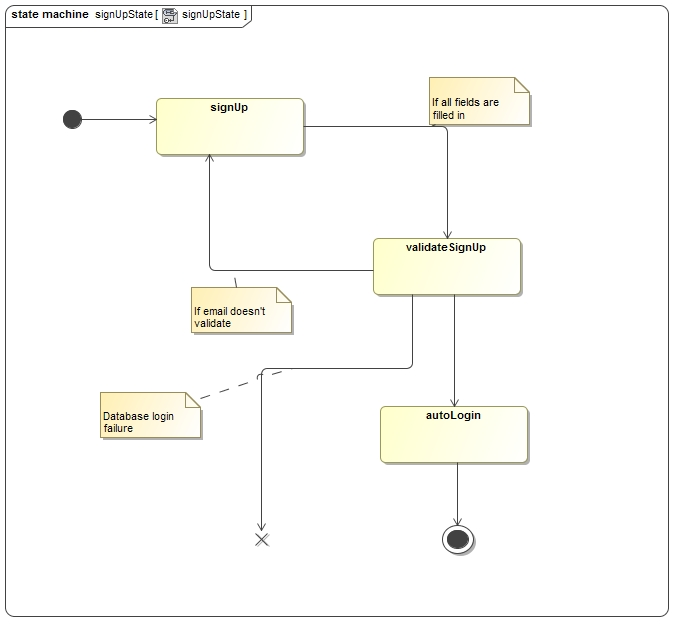
\includegraphics[width=15cm]{./graphics/signUpState.jpg}
    \caption{SignUp state diagram}
\end{figure}
\item Login\par
Priority: Critical.\par
Pre-condition: Client must have a STORM profile.\par
Post-condition: Client can now use STORM functionality.\par
\item Log out\par
Priority: Critical.\par
Pre-condition: Client must be logged into STORM.\par
\begin{figure}[H]
    \centering
    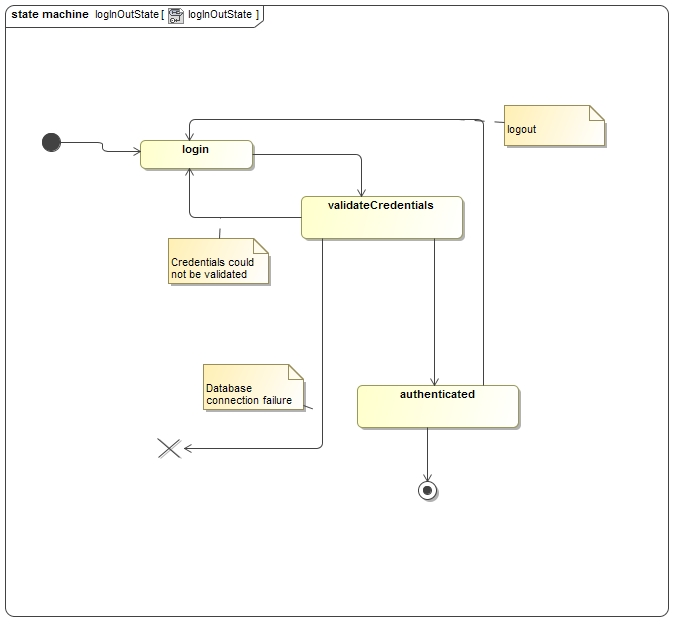
\includegraphics[width=15cm]{./graphics/logInOutState.jpg}
    \caption{Login/logout state diagram}
\end{figure}
\end{enumerate}


\subsection{Project Module}
This module deals with the configuration of projects. Initially a skeleton project will be set up with basic criteria 
and additional criteria can be added at a later stage as needed.
\subsubsection{Use-cases}
The projects mojule provides services create and manipulate projects.\par
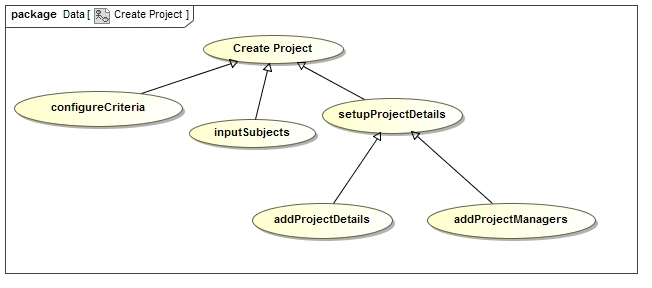
\includegraphics[width=13cm]{./graphics/createProjectUseCase.jpg}
    \rule{0\linewidth}{0.15\linewidth}\par
\begin{enumerate}
\item addProjectDetails\par
Priority: Critical.\par
Pre-condition: Client must be logged in.\par
Post-condition: Client must have a STORM profile.\par
Post-condition: Project skeleton is created in database.\par
\item addProjectManagers\par
Priority: Important.\par
Pre-condition: Client must have a STORM profile.\par
Pre-condition: Manager to be added must have a STORM profile.\par
Pre-condition: Client must have created a STORM project.\par
Post-condition: Manager has permition to colaborate on the project.\par
\item inputSubjects\par
Priority: Critical.\par
Pre-condition: Client must have a STORM profile.\par
Pre-condition: Client must have created a STORM project skeleton.\par
Post-condition: Project database is updated with a list of subjects.\par
\item ConfigureCriteria\par
Priority: Critical.\par
Pre-condition: Client must have a STORM profile.\par
Pre-condition: Client must be logged into STORM.\par
Pre-condition: Client must have created a STORM project skeleton.\par
Post-condition: Criteria for project is changed.\par
\end{enumerate}
\begin{figure}[h]
    \centering
    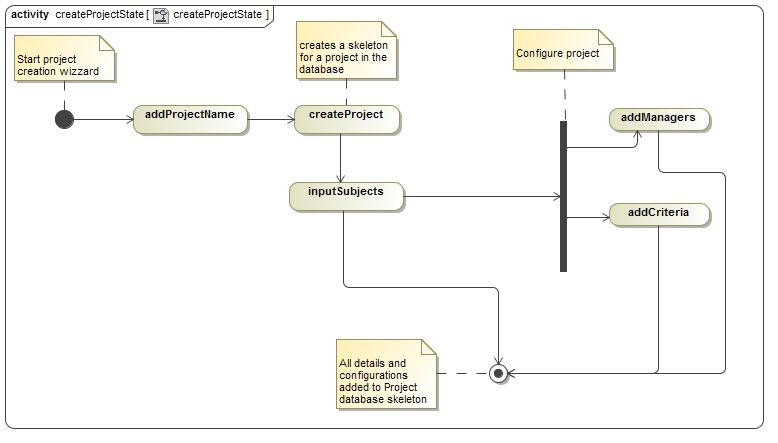
\includegraphics[width=15cm]{./graphics/createProjectState.jpg}
    \caption{createProject sate diagram}
    \label{fig:createProject_state}
\end{figure}
\subsection{Database Interaction Module}
include use cases here
\subsection{Algorithm Module}
This module deals with the main process behind STORM, it is the shuffling algorithm.

\subsubsection{Use-cases}
The algorithm module adds the functionality required to shuffle subjects into teams.\par
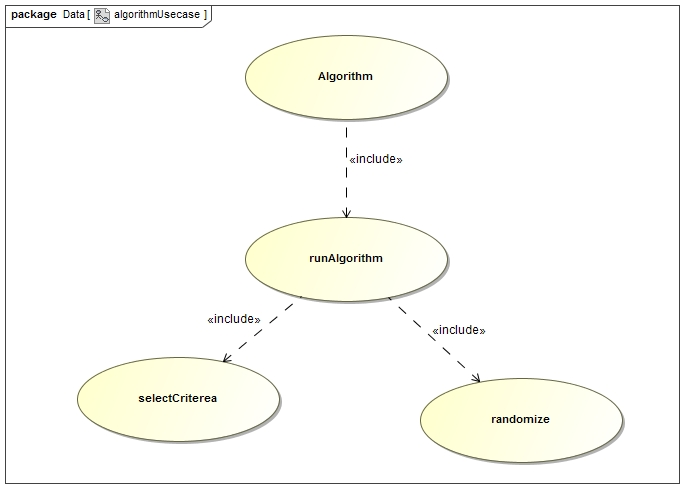
\includegraphics[width=13cm]{./graphics/algorithmUsecase.jpg}
    \rule{0\linewidth}{0.15\linewidth}\par

\begin{enumerate}
\item Randomize\par
Priority: Critical.\par
Pre-condition: Project must have users.\par
Pre-condition: Team size or number of teams must be specified.\par
Post-condition: Random teams are built.\par
    \begin{figure}
        \centering
        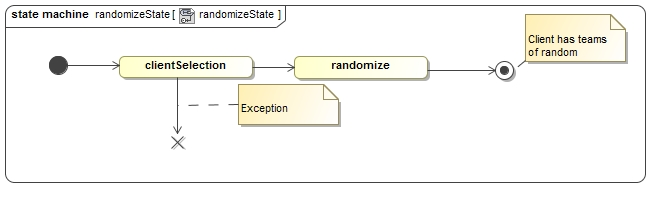
\includegraphics[width=13cm]{./graphics/randomizeState.jpg}
        \caption{Randomize state diagram}
        \label{fig:randomize_state}
    \end{figure}
\end{enumerate}
To be completed in future iterations
\pagebreak
\subsection{File Handling Module}
This section discusses the handling, parsing and validation of imported and exported .csv files.\par
\subsubsection{Use-cases}
The file handling module provides services to import, export and validate subject set files in .CSV format.\par
\begin{figure}[H]
    \centering
    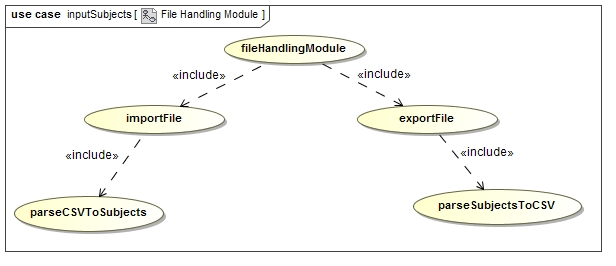
\includegraphics[width=15cm]{./graphics/fileUseCase.jpg}
    \caption{File Handling Module Use Case}
\end{figure}
\begin{enumerate}
\item parseCSVToSubjects\par
Priority: Critical\par
Pre-condition: The input file must pass the validation tests.\par
Post-condition: Subject set is modified locally.\par
\item saveSubjectsToDatabase\par
Priority: Critical.\par
Pre-condition: The user must click on the save button.\par
Pre-condition: The subject set needs to be locally modified.\par
Post-condition: The subject set is saved to the database.\par
\item parseSubjectsToCSV\par
Priority: Critical.\par
Pre-condition: The subject set must exist in the database.\par
Pre-condition: The correct format should be generated.\par
Pre-condition: The user must have enough hard disk space to save the .CSV file.\par
Post-condition: A CSV file with all the subjects existing in the project is downloaded to the user's hard drive .\par

\end{enumerate}
\end{document}
